%%%%%%%%%%%%%%%%%%%%%%%%%%%%%%%%%% PREAMBULO %%%%%%%%%%%%%%%%%%%%%%%%%%%%%%%%%%%%%%

\documentclass[%
    %draft,%
    a4paper,%
    12pt,%
    %oneside,%
    twoside,%
    openright,%
    halfparskip,%
    cleardoubleempty,%
    bigheadings,%
    %tocleft,
    titlepage,%
    %fleqn,%
    headsepline%
]{scrbook}

%\usepackage[lmargin=3.5cm,rmargin=1.7cm,tmargin=3.85cm,bmargin=4.5cm]{geometry}
\typearea{12}


\usepackage[T1]{fontenc}%encoding de los fonts del pdf (para copiar y pegar)
\usepackage[utf8]{inputenc} %encoding del .tex
\usepackage[spanish]{babel} %idioma español para los cortes de linea
\usepackage{amsmath} %paquete de matematica
% \usepackage[margin=2cm]{geometry} %margenes
\usepackage{enumerate} %mejor enumerate
\usepackage{xspace} %espacios despues de un comando
\usepackage{listings} %para escribir codigo C++
\usepackage{graphicx} % figuras
\usepackage[pdftitle={},pdfauthor={},pdfcreator={},pdfsubject={},pdfkeywords={},colorlinks=true,linkcolor=blue,citecolor=blue]{hyperref} %hiperlinks
\usepackage{amsmath,amsthm,amssymb} %matematica

\newtheorem{theorem}{Teorema}

\newcommand{\Grafo}{\textsc{Grafo}\xspace}
\newcommand{\Code}[1]{\lstinline[basicstyle={\tt}]@#1@}
\newcommand{\N}{\mathcal{N}}

\lstset{
  numbers=left,
  numberstyle=\small,
  tabsize=2,
  frame=BRtl,
  basicstyle={\small\tt},
  aboveskip={12pt},
  belowskip={12pt},
  captionpos=b,
  framerule=1.5pt,
  %linewidth=.9\linewidth
  xleftmargin=3em,
  xrightmargin=3em,
  emphstyle={\color{red}}
}


\begin{document}

%%%%%%%%%%%%%%%%%%%%%%%%%%%%%%%%%%% CARATULA %%%%%%%%%%%%%%%%%%%%%%%%%%%

\frontmatter
\begin{titlepage}

\vspace*{\stretch{1}}

\begin{center}

\includegraphics[width=9cm, keepaspectratio]{./logo-unq.jpg}\\

\medskip

Departamento de Ciencia y Tecnología\\
Tecnicatura Universitaria en Programación Informática\\

\vspace{3cm}

\textbf{\huge Implementación de la estructura $h$-grafo}\\[0.4cm] 

\vspace{1.5cm}

{\large \bf \hspace{\stretch{3}}Griselda Cardozo\hspace{\stretch{1}}Alejandro Merlo\hspace{\stretch{3}}}

\end{center}

\vspace{3cm}

\textbf{Director:} Dr. Francisco Soulignac

\vspace{5mm}

Bernal, \today
\vspace*{\stretch{2}}
\end{titlepage}


\newpage

%%%%%%%%%%%%%%%%%%%%%%%%%%%%% RESUMEN %%%%%%%%%%%%%%%%%%%%%%%%%%%%

%Opcion para doble faz
\thispagestyle{empty} \cleardoublepage

\thispagestyle{empty}

\vspace*{2cm}

\begin{center}
\Large \textbf{Implementación de la estructura $h$-grafo}
\end{center}

\vspace*{\stretch{1}}

Poner aca un resumen

\noindent \textbf{Palabras clave:} \textit{$h$-grafo, grafos ralos, arboricidad, implementación.}

\vspace*{\stretch{2}}
\newpage
%Opcion para doble faz
\thispagestyle{empty} \cleardoublepage



%%%%%%%%%%%%%%%%%%%%%%%%%% DEDICATORIA Y AGRADECIMIENTOS %%%%%%%%%%%%%%%%%%%%%%

\vspace*{\stretch{1}}
{\raggedleft\emph{Para quien sea.\\ Alguna frase si queres\\Griselda Cardozo.}\par
            \emph{Para quien sea.\\ Alguna frase si queres\\Alejandro Merlo.}\par}
\vspace*{\stretch{1}}

%Opcion para doble faz
\thispagestyle{empty} \cleardoublepage

\chapter*{Agradecimientos}

A quien corresponda, o se elimina

\hspace*{\stretch{1}} Fecha del dia del agradecimiento.

%Opcion para doble faz
\thispagestyle{empty} \cleardoublepage

\tableofcontents

\mainmatter

\chapter{Introducción}
\label{sec:introduccion}

Los grafos son estructuras abstractas que sirven para modelar distintas tipos de relaciones matemáticas.  Formalmente, un \emph{grafo} es un par $G = (V, E)$ donde $V$ es un conjunto (finito) de \emph{vértices} y $E$ es un conjunto formado por pares de vértices.  En términos matemáticos, los vértices son objetos cuya única propiedad es la de ser distinguibles; en la práctica, los vértices representan objetos de algún dominio de aplicación.  Los pares $(v,w)$ que pertenecen a $E$ son llamados \emph{aristas}, y su propósito es reflejan alguna relación entre $v$ y $w$.  Los grafos se usan para modelar relaciones de problemas reales en forma abstracta.  Por ejemplo, una red social se modela con un grafo que tiene un vértice por cada persona y una arista entre dos vértices para indicar que las personas son amigas.  La ventaja de utilizar grafos en lugar de los objetos que ellos modelan, es que tenemos acceso a una terminología común, de manera tal que podemos traducir los avances de una aplicación a otra.  De esta forma, podemos aprovechar la teoría de grafos para resolver problemas de areas tan diversas como las matemáticas discretas, la infórmatica, las telecomunicaciones, la biología, la sociología, la filosofía, etc.~\cite{GrossYellen2006}.  La \emph{teoría de grafos} es la disciplina que se encarga del estudio de grafos, mientras que la teoría \emph{algorítmica} de grafos se encarga de los problemas computacionales asociados.

El objetivo del presente trabajo es implementar la estructura de datos $h$-grafo descrita por Lin et al.~\cite{LinSoulignacSzwarcfiterTCS2012}.   Como objetivos particulares de nuestro desarrollo, esperamos:
\begin{itemize}
  \item Verificar la correctitud de la misma.  Si bien el artículo describe la estructura con suficiente detalle, la misma no está implementada en un lenguaje de programación real.  En consecuencia, podrían haber detalles de implementación no detectados a la hora de describir la estructura.
  \item Analizar la dificultad de implementar la estructura en un lenguaje eficiente de escala industrial.  Como es común en los artículos de investigación teóricos, los investigadores suponen la existencia de ciertas tipos de datos (como las listas) con una interfaz apropiada a sus objetivos.  Sin embargo, las implementaciones reales de las mismas muchas veces distan de dicha interfaz ideal, lo que obliga a re-implementar estructuras básicas (e.g., re-implementar listas para tener acceso a la representación interna) o a resolver las discrepancias usando las estructuras ya existentes (e.g., utilizar \emph{iteradores} como si fueran punteros a los nodos de la representación).  En este trabajo tomamos la segunda opción.
\end{itemize}
Como objetivo futuro, que excede el alcance del trabajo realizado, sería deseable también analizar la eficiencia de la estructura de datos, tanto de forma aislada como en comparación con otras estructuras.

La estructura $h$-grafo se usa para implementar el \emph{tipo abstracto de datos} (TAD) \Grafo, que es una representación computacional del correspondiente objeto matemático.  De acuerdo a la interfaz que uno elija para operar con un grafo, es posible definir distintos tipos de TADs, con distintas características, que sean más o menos útiles para las distintas aplicaciones.  En particular, la estructura $h$-grafo fue concebida para aplicaciones que requieren grafos dinámicos.  Por \emph{dinámico} nos referimos a que la interfaz debe proveer operaciones eficientes para insertar y borrar vértices y aristas, a la vez que provee operaciones eficientes de consulta.  Es por este motivo que el TAD \Grafo que nosotros presentamos es consistente con el dinamismo requerido por las aplicaciones.  

La estructura $h$-grafo es una estructura general que se puede usar para representar a cualquier grafo.  Sin embargo, la estructura es particularmente eficiente en grafos \emph{ralos}, i.e., grafos con pocas aristas.  Existen distintas definiciones de dan cuenta de qué es un grafo ralo.  La definición más básica (y general) establece que un grafo es ralo cuando tiene $O(n)$ aristas, siendo $n$ la cantidad de vértices del grafo.  Si bien esta noción es útil, el resultado es que cualquier grafo no-ralo se puede convertir en un grafo ralo agregando suficiente vértices de grado bajo.  En muchas aplicaciones, estos vértices se pueden preprocesar eficientemente, lo que nos deja con un grafo no-ralo.  En particular, la estructura $h$-grafo requiere, para ser eficiente, que cualquier parte del grafo sea rala.  En otras palabras, la estructura es eficiente cuando todo subgrafo con $k$ vértices tiene $O(k)$ aristas.  Esta es la noción que nosotros vamos a considerar cuando decimos que un grafo es ralo.  En particular, Nash-Williams~\cite{Nash-WilliamsJLMS1964} observo que un grafo es ralo baja, razón por la cual el artículo de Lin et al.~\cite{LinSoulignacSzwarcfiterTCS2012} utiliza el parámetro de la arboricidad para analizar la eficiencia de los algoritmos.  Vale remarca que la arboricidad de un grafo con $m$ aristas es a lo sumo $O(\sqrt{m})$, y que los grafos planares tienen arboricidad $3$.  

Los objetivos específicos de este este trabajo son:
\begin{enumerate}
  \item describir una interfaz apropiada para el TAD \Grafo, siguiendo los usos y costumbres de nuestro lenguaje de implementación (C++),
  \item desarrollar el TAD grafo implementado con la estructura $h$-grafo, aprovechando la biblioteca estándar de nuestro lenguaje,
  \item verificar que la eficiencia teórica coincide con la de nuestra implementación para algunos grafos, y
  \item probar la eficiencia de la estructura en algunos grafos ralos grandes.
\end{enumerate}
Como objetivo a futuro quedará el análisis de la estructura en aplicaciones reales de gran escala.

El presente documento esta organizado de la siguiente forma.  En el Capítulo~\ref{sec:tad grafo} describimos el TAD \Grafo, desde un punto de vista agnóstico con respecto al lenguaje, haciendo un repaso de su interfaz.  En el Capítulo \ref{sec:h-grafo} explicamos la estructura $h$-grafo, a la vez que describiremos los diferentes algoritmos que implementan las distintas operaciones del TAD \Grafo.  Este Capítulo también está presentado en forma independiente al lenguaje.  Luego, en el Capítulo~\ref{sec:c++}, nos centraremos en la implementación del TAD usando el lenguaje C++. Este capítulo está dividido en dos secciones. La primera, Sección~\ref{sec:c++:interfaz}, da cuenta de la interfaz del $h$-grafo siguiendo los lineamientos de C++. La segunda, Sección~\ref{sec:c++:estructura}, explica cómo se implementa la estructura en C++ aprovechando la biblioteca estándar.  El Capítulo~\ref{sec:experimentación} presenta brevemente algunos resultados en los que medimos la eficiencia de la estructura $h$-graph.  Finalmente, el Capítulo~\ref{sec:final} presenta un breve resumen de lo logrado junto con las posibilidades de desarrollo a futuro.

\section{Preliminares}
\label{sec:definiciones}

Como mencionamos en la sección anterior, el objetivo central de este trabajo es implementar un TAD \Grafo que explote la estructura de datos $h$-grafo.  El TAD \Grafo es una representación computacional del objeto abstracto \emph{grafo}, que es el que se estudia en teoría de grafos.  En esta sección incluimos definiciones de la teoría de grafos que son necesarias para comprender nuestro trabajo (ver Figura~\ref{fig:definiciones} en donde se ejemplifican muchas de las definiciones de esta sección).

%Definiciones matematicas
Un \emph{grafo} es un par $G = (V, E)$ donde $V$ es un conjunto finito de \emph{vértices} y $E$ es un conjunto de pares no ordenados, llamados \emph{aristas}.  Vamos a escribir $V(G)$ y $E(G)$ para denotar a $V$ y $E$, mientras que al par no ordenado formado por $v$ y $w$ lo vamos a escribir como $vw$.  Para cada $vw \in E$, decimos que $v$ y $w$ son \emph{vecinos} o \emph{adyacentes}.  El grado $d(v)$ de un vértice $v$ es la cantidad de vecinos que tiene $v$.  El $k$-vecindario de $v$ es el conjunto $N(v, k)$ de todos los vecinos de $v$ que tienen grado $k$, para algun $k \in \mathbb{N}$.  Obviamente, $N(v,k) = \emptyset$ para todo $k \geq n$.  Al conjunto $N(v)$ de todos los vecinos de $v$ lo llamamos, simplemente, su \emph{vecindario}.  Notar que $N(v)$ es la unión de todos los $k$-vecindarios de $v$, i.e., $N(v) = \bigcup_{i=0}^{n-1}N(v,k)$.

Un grafo $H$ es un \emph{subgrafo} de $G$ cuando $V(H) \subseteq V(G)$ y $E(H) \subseteq E(G)$.  Si $V(H) = V(G)$, entonces $H$ es un subgrafo \emph{generador} de $G$.  Un \emph{camino} de $G$ es una secuencia de vértices distintos $v_1, \ldots, v_k$ tal que $v_iv_{i+1} \in E(G)$ para todo $1 \leq i < k$.  Un ciclo es una secuencia $v_1, \ldots, v_k, v_1$ tal que $v_1, \ldots, v_k$ es un camino.  Los \emph{bosques} son aquellos grafos que no tienen ciclos.  La \emph{arboricidad} $\alpha(G)$ de un grafo $G$ es la mínima cantidad de bosques generadores en las que se puede particionar $E(G)$.  Los siguientes resultados relacionan la arboricidad de $G$ con su cantidad de aristas.

\begin{theorem}[\cite{Nash-WilliamsJLMS1964}]
  Para todo grafo $G$ ocurre que
  \[\alpha(G) = \max\left\{\frac{|E(H)|}{|V(H)|-1} \middle| H \text{ es subgrafo de }G\right\}\]
\end{theorem}

\begin{theorem}[\cite{ChibaNishizekiSJC1985}]
  Para todo grafo $G$ ocurre que $\alpha(G) \leq 2\sqrt{m}$.
\end{theorem}




\begin{figure}
  \centering
  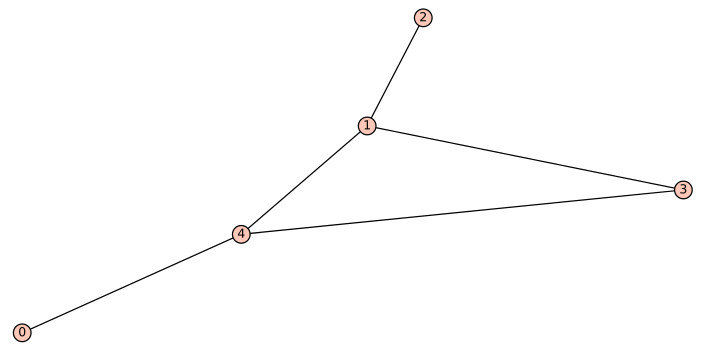
\includegraphics[width=0.8\textwidth]{./grafo.jpeg}
  \fbox{Figura de un grafo en el que mostramos las definiciones}

  \caption{Grafo $G$ con $V(G) = \{0,1,2,3,4\}$ y $E(G) =\{(0,4),(1,2),(1,3),(1,4),(3,4)\}$.  El vértice $1$ tiene grado $3$ y su vencindario es $\{2,3,4\}$. La secuencia $0, 4, 1, 2$ es un camino, mientras que $4,1,3,4$ es un ciclo.  El grafo $H$ con $V(H) = V(G)$ y $E(H) = \{04, 13, 12\}\}$ es un bosque que es subgrafo generador de $G$, i.e., $H$ es un bosque generador de $G$.  Como \{$H$, $J$\} es una partición en bosques de $G$, con $V(J) = V(G)$ y $E(J) = E(G) \setminus E(H)$, entonces $\alpha(G) \leq 2$.  Más aún, $\alpha(G) = 2$ porque $G$ no se puede particionar en un único bosque (ya que no es un bosque).}\label{fig:definiciones}
\end{figure}


\chapter{El tipo abstracto \Grafo}
\label{sec:tad grafo}

\def\lstlistingname{Pseudocódigo}
 
El propósito de esta sección es presentar la interfaz del tipo abstracto \Grafo que implementaremos.  Cada instancia de este TAD es \emph{dinámica}, en el sentido que la instancia va mutando de acuerdo la inserción de vértices y aristas.  Asimismo, el TAD ofrece distintas operaciones de consulta, que están pensadas para poder recorrer eficientemente el vecindario de las distintas aristas del grafo.  Estas operaciones son muy útiles, por ejemplo, cuando uno quiere analizar la estructura ``local'' del grafo.  Es decir, cómo se conectan los vecinos de un vértice $v$ dado entre sí.  

Para describir la interfaz del TAD \Grafo, vamos a detallar cada una de las operaciones junto con sus propósitos y sus requerimientos (precondiciones).  Esta descripción será de alto nivel, tal y como se desarrolla en~\cite{LinSoulignacSzwarcfiterTCS2012}.  La idea de esta sección es fijar los conceptos necesarios para la posterior descripción de su implementación en el lenguaje C++.  Asimismo, mostraremos ejemplos  de uso de las distintas operaciones y describiremos la complejidad temporal esperada.  Obviamente, esta complejidad está en función de la implementación que se pospone al Capítulo~\ref{sec:h-grafo}.  
% * <griseldavcardozo@gmail.com> 2016-01-17T19:15:12.371Z:
%
% Arriba hay una cita y no sé que poner
%
% ^ <griseldavcardozo@gmail.com> 2016-01-17T19:15:40.671Z.

Recordemos que si bien los vértices de un grafo son elementos abstractos, los mismos se usan para representar entidades de aplicaciones reales.  Es común que estas entidades tengan alguna información propia que es requerida dentro de la aplicación.  Es por este motivo que el grafo permite asociar cierta información a cada vértice, lo que convierte al TAD \Grafo en un tipo paramétrico.  Específicamente, el TAD \Grafo almacena objetos de un tipo un tipo genérico \texttt{elem}.

\section{\texttt{create\_graph()}}
\label{sec:tad grafo:create-graph}

Crea un objeto \Code{G} que representa un grafo $G$ de elementos \Code{elem}. Retorna un puntero \Code{G} al nuevo grafo creado. Este objeto guarda cierta información correspondiente a los vértices y sus vecinos. El \lstlistingname~\ref{lst:pseudo:create_graph} muestra cómo crear un grafo $G$ vacío.


\begin{description}
  \item [Propósito:] crea un \Code{G} sin vertices ni aristas.
  \item [Retorna:] un puntero \Code{G} al grafo $G$.
  \item [Complejidad temporal: O(1)]
\end{description}


\begin{lstlisting}[caption={Ejemplo de uso de \Code{create\_graph}},gobble=2,float=ht,label={lst:pseudo:create_graph},emph={create_graph}]
  G := create_graph()
\end{lstlisting}

\subsection{\texttt{insert\_vertex(G, info)}}
\label{sec:tad grafo:insert-vertex}

Modifica un objeto \Code{G} que representa un grafo $G$, a fin de representar el grafo $H$ que se obtiene de insertar un nuevo vértice $v$ en $G$.  A este vértice $v$ se le puede asociar cierta información que es la reflejada por el parémetro \Code{info}.  Retorna un puntero \Code{v} al nuevo vértice $v$ agregado.  Este puntero \Code{v} debe usarse para interactuar con $G$ a fin de modificar sus propiedades.  Notar que el puntero \Code{v} es un objeto conocido sólo por \Code{G} y no es compartido con otras instancias del TAD Grafos.  En particular, el uso de \Code{v} con otra instancia que no sea \Code{G} conduce a un comportamiento indefinido.  

El \lstlistingname~\ref{lst:pseudo:insert_vertex} muestra cómo usar \texttt{insert\_vertex}.
  
\begin{description}
  \item [Parámetros:] \Code{G} representa un grafo $G$ e \Code{info} es cualquier objeto.
  \item [Propósito:] modifica \Code{G} para representar un grafo $G + v$.
  \item [Retorna:] un puntero \Code{v} al vértice $v$.
  \item [Complejidad temporal: O(n)]
\end{description}


\begin{lstlisting}[caption={Ejemplo de uso de insert\_vertex.  Crea un grafo $G$ con dos vértices, ambos con la letra ``a'' como información.  Luego, el ciclo imprime ``aa''. Ver Sección~\ref{sec:tad grafo:vertex-iterator} para más información de \texttt{vertex\_iterator}.},gobble=2,float=ht,label={lst:pseudo:insert_vertex},emph={insert_vertex}]
  G := create_graph()
  v := insert_vertex(G, `a')
  w := insert_vertex(G, `a')
  for v in vertex_iterator(G):
      print get_info(v)
\end{lstlisting}


\subsection{\texttt{remove\_vertex(G, v)}}
\label{sec:tad grafo:remove-vertex}

Modifica un objeto \Code{G} que representa un grafo $G$, a fin de representar el grafo $H$ que se obtiene de remover el vértice existente \Code{v} que representa al vértice $v$ en $G$.  Como resultado de esta operación, se invalidan aquellos iteradores que están relacionados con $v$ (es decir: iteradores de vértices que apuntan a $v$, iteradores de vecindarios de $v$, iteradores de vecindarios de cualquier vértice $w \in N(v)$ que circunstancialmente este recorriendo a $v$, e iteradores de vecindarios que circunstancialmente esten recorriendo algún $w \in N(v)$).
  
\begin{description}
  \item [Parámetros:] \Code{G} representa un grafo $G$ y \Code{v} representa un vértice existente $v$ de $G$.
  \item [Propósito:] modifica \Code{G} para representar un grafo $G - v$.
  \item [Complejidad temporal: O(n)]
\end{description}


\begin{lstlisting}[caption={Ejemplo de uso de remove\_vertex. El código crea un grafo $G$ con dos vértices, el primero \texttt{v} representa al vértice $v$ con la letra 'a' y el segundo \texttt{w} representa al vértice $w$ con la letra 'b' como infomación. Luego, remueve \texttt{v} del grafo y el ciclo imprime ``b'' como resultado. Ver Sección~\ref{sec:tad grafo:vertex-iterator} para más información de \texttt{vertex\_iterator}.},gobble=2,float=ht,label={lst:pseudo:remove_vertex},emph={remove_vertex}]
  G := create_graph()
  v := insert_vertex(G, 'a')
  w := insert_vertex(G, 'b')
  remove_vertex(G, v)
  for vt in vertex_iterator(G):
      print get_info(vt)
\end{lstlisting}


\subsection{\texttt{add\_edge(G, v, w)}}
\label{sec:tad grafo:add-edge}

Modifica un objeto \Code{G} que representa un grafo $G$, a fin de representar el grafo $H$ que se obtiene de agregar la arista $vw$ conformada por \Code{v} y \Code{w} que representan los vértices $v$ y $w$ en $G$.


\begin{description}
  \item [Parámetros:] \Code{G} representa un grafo $G$, \Code{v} y \Code{w} representan los vértices existentes $v$ y $w$ de $G$.
  \item [Propósito:] modifica \Code{G} para representar un grafo $G + vw$.
  \item [Complejidad temporal:]
\end{description}


\begin{lstlisting}[caption={Ejemplo de uso de add\_edge. El código crea un grafo $G$ con dos vértices, el primero \texttt{v} representa al vértice $v$ con el número 1 y el segundo \texttt{w} representa al vértice $w$ con el número 2 como infomación. Luego, crea la arista $vw$ entre estos dos vértices dentro del grafo $G$. El ciclo imprime cada uno de los valores de los vecinos de $v$, en este caso como $w$ es su único vecino imprime ``2''. Ver Sección~\ref{sec:tad grafo:neighbor-iterator} para más información de \texttt{neghbor\_iterator}.},gobble=2,float=ht,label={lst:pseudo:add_edge},emph={add_edge}]
  G := create_graph()
  v := insert_vertex(G, 1)
  w := insert_vertex(G, 2)
  add_edge(G, v, w)
  for n in neighbor_iterator(v):
      print get_info(n)
\end{lstlisting}


\subsection{\texttt{remove\_edge(G, v, w)}}
\label{sec:tad grafo:remove-edge}

Modifica un objeto \Code{G} que representa un grafo $G$, a fin de representar el grafo $H$ que se obtiene de remover la arista $vw$ conformada por \Code{v} y \Code{w} que representan los vértices $v$ y $w$ en $G$.
Como resultado de esta operación, se invalidan aquellos iteradores de vecindarios que están relacionados con $v$ o $w$ (es decir:  iteradores de vecindarios de $v$ o $w$, e iteradores de vecindarios de otros vértices que circunstancialmente estén recorriendo algún $z \in N(v) \cup N(w)$).

\begin{description}
  \item [Parámetros:] \Code{G} representa un grafo $G$, \Code{v} y \Code{w} representan vértices adyacentes $v$ y $w$ de $G$, respectivamente.
  \item [Propósito:] modifica \Code{G} para representar un grafo $G - \{vw\}$.
  \item [Complejidad temporal:]
\end{description}


\begin{lstlisting}[caption={Ejemplo de uso de \Code{remove_edge}.  En el código se crea un grafo $G$ con vértices $v$, $w$ y $x$, siendo $v$ adyacente tanto a $w$ como a $x$.  Luego se utiliza \Code{remove_edge} para eliminar la arista $vw$, con lo cual $v$ queda adyacente únicamente a $x$.  El ciclo final, pues, imprime el valor $3$ asociado a $x$.  Ver Sección~\ref{sec:tad grafo:neighbor-iterator} para más información de \Code{neghbor_iterator}.},gobble=2,float=ht,label={lst:pseudo:remove_edge},emph={remove_edge}]
  G := create_graph()
  v := insert_vertex(G, 1)
  w := insert_vertex(G, 2)
  x := insert_vertex(G, 3)
  add_edge(G, v, w)
  add_edge(G, v, x)
  remove_edge(G, v, w)
  for n in neighbor_iterator(v):
      print get_info(n)
\end{lstlisting}


\subsection{\texttt{add\_vertex(G, info, N)}}
\label{sec:tad grafo:add-vertex}

Modifica un objeto \Code{G} que representa un grafo $G$, a fin de representar el grafo $H$ que se obtiene de agregar un nuevo vértice $v$ cuya información está reflejada en el parámetro \Code{info} y una lista de punteros \Code{N} que representa al vecindario $N$ que será asociado a $v$

\begin{description}
  \item [Parámetros:] \Code{G} representa un grafo $G$, \Code{info} es cualquier objeto y \Code{N} representa el vecindario $N$.
  \item [Propósito:] modifica \Code{G} para representar un grafo $G + vn$ donde $n$ es cada elemento de $N$.
  \item [Retorna:] un puntero \Code{v} al vértice $v$.
  \item [Complejidad temporal: O(1)]
\end{description}


\begin{lstlisting}[caption={Ejemplo de uso de \Code{add_vertex}. El código crea un grafo $G$ con tres vertices, teniendo el tercer vertice, llamado $v$, a los otros dos como vecinos. Luego, el ciclo imprime ``12''.},gobble=2,float=ht,label={lst:pseudo:add_vertex},emph={add_vertex}]
  G := create_graph()
  x := insertVertex(G, 1);
  y := insertVertex(G, 2);
  v := add_vertex(G, 3, {x, y})
  for w in neighbor_iterator(v):
      print get_info(w)
\end{lstlisting}


\subsection{\Code{vertex_iterator(G)}}%iterador
\label{sec:tad grafo:vertex-iterator}

Provee de un puntero que permite desplazarse a través de los distintos vertices del objeto \texttt{G} que representa un grafo $G$ y acceder a ellos, a fin de poder manipularlos de una forma rápida y simple.

\begin{description}
  \item [Parámetros:] \Code{G} representa un grafo $G$.
  \item [Propósito:] proveer al usuario de un mecanismo para iterar los vertices de $G$.
  \item [Retorna:] un iterador \Code{i} a los vértices de $G$.
  \item [Complejidad temporal:]
\end{description}


\begin{lstlisting}[caption={Ejemplo de uso de \Code{vertex_iterator}. El código crea un grafo $G$ con el vertice 1 y el vertice 2. Luego, mediante el iterador de $G$ se recorre sus vertices y el ciclo imprime ``12''.},gobble=2,float=ht,label={lst:pseudo:vertex_iterator},emph={vertex_iterator}]
  G := create_graph()
  x := insertVertex(G, 1);
  y := insertVertex(G, 2);
  for v in vertex_iterator(G):
      print get_info(v)
\end{lstlisting}


\subsection{\Code{neighbor_iterator(v)}}%iterador
\label{sec:tad grafo:neighbor-iterator}

Provee de un puntero que permite desplazarse a través de los vecinos del vértice $v$ representado por el objeto \texttt{v}, a fin de acceder y manipular cada vecino de forma rápida y simple.  Si bien no está implementado en esta versión, dicho iterador tambien podría usarse para eliminar directamente la arista entre $v$ y $w$ para cada $w \in N(v)$ que se recorre.

\begin{description}
  \item [Parámetros:] \Code{v} representa un vértice $v$.
  \item [Propósito:] proveer al usuario de un mecanismo para iterar los vecinos de $v$.
  \item [Retorna:] un iterador \Code{i} a los vecinos de menor grado de $v$.
  \item [Complejidad temporal:]
\end{description}


\begin{lstlisting}[caption={Ejemplo de uso de neighbor\_iterator. El código crea un grafo $G$ con el vértice 1, el vértice 2 y el vértice 3. Luego, mediante el iterador de $v$ se recorre sus vecinos de menor grado y el ciclo imprime ``12''.},gobble=2,float=ht,label={lst:pseudo:neighbor_iterator},emph={neighbor_iterator}]
  G := create_graph()
  x := insertVertex(G, 1);
  y := insertVertex(G, 2);
  v := add_vertex(G, 3, {x, y})
  for w in neighbor_iterator(v):
      print get_info(w)
\end{lstlisting}


\subsection{\Code{H_neighbor_iterator(v)}}%iterador
\label{sec:tad grafo:H-neighbors}

Provee de un puntero que permite desplazarse a través de los distintos vecinos de grado mayor o igual al vértice $v$ representado por el objeto \texttt{v}, a fin de poder acceder y manipular cada vecino de forma rápida y simple.  Si bien no está implementado en esta versión, dicho iterador tambien podría usarse para eliminar directamente la arista entre $v$ y $w$ para cada $w \in N(v)$ que se recorre.

\begin{description}
  \item [Parámetros:] \Code{v} representa un vértice $v$.
  \item [Propósito:] proveer al usuario de un mecanismo para iterar los vecinos de grado mayor o igual al de $v$.
  \item [Retorna:] un iterador \Code{i} a los vecinos de grado mayor o igual al de $v$.
  \item [Complejidad temporal:]
\end{description}


\begin{lstlisting}[caption={Ejemplo de uso de \Code{H_neighbor_iterator}. El código crea un grafo $G$ con el vértice 1, el vértice 2 y el vértice 3. Luego, mediante el iterador de $x$ se recorre sus vecinos de mayor o igual grado y el ciclo imprime ``3''.},gobble=2,float=ht,label={lst:pseudo:H_neighbors},emph={H_neighbors}]
  G := create_graph()
  x := insertVertex(G, 1);
  y := insertVertex(G, 2);
  v := add_vertex(G, 3, {x, y})
  for w in H_neighbor_iterator(x):
      print get_info(w)
\end{lstlisting}


\subsection{\Code{degree(v)}}
\label{sec:tad grafo:degree}

Dado un objeto \Code{v} que representa un vértice $v$ devuelve la cantidad de vecinos de dicho vértice. 

\begin{description}
  \item [Parámetros:] \Code{v} representa un vértice $v$.
  \item [Retorna:] un número que denota la cantidad de vecinos de $v$.
  \item [Complejidad temporal: O(1)]
\end{description}


\begin{lstlisting}[caption={Ejemplo de uso de degree. El código crea un grafo $G$ con el vértice 1, el vértice 2 y el vértice 3. Luego se imprime el grado de $v$, es decir, ``2''.},gobble=2,float=ht,label={lst:pseudo:degree},emph={degree}]
  G := create_graph()
  x := insertVertex(G, 1);
  y := insertVertex(G, 2);
  v := add_vertex(G, 3, {x, y})
  print degree(v)
\end{lstlisting}


\chapter{La estructura $h$-grafo}
\label{sec:h-grafo}

En esta sección describimos la estructura $h$-grafo que usamos para implementar el TAD grafo descripto en la Seccion~\ref{sec:tad grafo}.  Esta estructura es particularmente apropiada para grafos ralos, i.e., grafos cuya arboricidad es baja.  Esto se ve reflejado en  las complejidades temporales esperadas, dado que las mismas dependen de la cantidad de aristas y la arboricidad del grafo.  La descripción la hacemos a alto nivel tal como en el paper.  La idea es explicar, a continuación, como esta compuesta la estructura interna del $h$-grafo y luego detallar cada uno de sus operaciones.


Conceptualmente, la estructura mantiene un objeto \texttt{v} para cada vértice $v$ del grafo $G$.  Este objeto \emph{representa} a $v$ y mantiene la tripla $(d(v), N(v), H(v))$.  Recordemos que:   
\begin{itemize}
\item $d(v)$ se refiere al grado del vértice
\item $N(v)$ representa a los vecinos de $v$ que tienen menor grado que $v$
1\item $H(v)$ representa a los vecinos de $v$ que tienen al menos el grado de $v$.
\end{itemize}

 Obviamente $d(v)$ se representa usando un número. Para representar $N(v)$, el $h$-grafo mantiene (ver Figura) una lista con objetos que representan vecinos que tienen igual grado entre sí. Cada uno de estos vecinos, llamémoslo $w$,  guarda un puntero a la lista $H(w)$ y otro puntero al lugar exacto dónde esta $v$ en $H(w)$.

Vale remarcar que los vértices son privados del grafo, en el sentido de que no se pueden manipular directamente.  En su lugar, el usuario modifica $v$ a través de un \emph{puntero} que obtiene al insertar el vértice (ver ~\ref{sec:tad grafo:vertex-iterator} ).  Remarcamos que este puntero es un objeto inteligente en el sentido que no muestra la implementacion al usuario.

En el resto de esta sección describimos cómo implementar, usando la estructura $h$-grafo, cada una de las operaciones que el TAD Grafo soporta (ver Seccion~\ref{sec:tad grafo}).  Para que quede claro que estamos usando la estructura $h$-grafo, vamos a escribir cada operacion \texttt{oper(G, $\cdots$)} usando la notación punto, i.e., \texttt{G.oper($\cdots$)} a fin de remarcar que tenemos acceso a la estructura de \texttt{G}.

En esta sección se describirá el algoritmo para insertar aristas y vértices y el algoritmo para removerlos.
Cómo se dijo anteriormente, la estructura del $h$-graph consiste de tres elementos, $d(v)$ que es el grado del vértice, $N(v)$ es una lista de sublistas que representa al vecindario de $v$, cada sublista no vacía contiene a los vecinos de determinado grado. Las sublistas están ordenadas. $H(v)$ es una la lista que contiene a los vecinos que tienen al menos el grado de $v$.

$h$-graph mantiene un puntero directo a los objetos que representan a los vértices, aristas y listas.


\subsection{\texttt{G.insert\_vertex(N, info)}}
\label{sec:hgraph:insert_vertex}

%IDEA
El proceso para insertar un nuevo vértice $v$ en $G$ se divide en dos partes.  Primero, la inserción de un nuevo objeto $v$ que representa un vértice aislado.  Segundo, la inserción de una arista entre $v$ y cada uno de los vértices representados por $N$.  Claramente, el grafo obtenido representa a $G + v$.

\subsubsection*{Pseudocódigo}

\begin{lstlisting}[float=h]
G.insert_vertex(N, info):
    v := G.append((0, [], []))
    for w in N:
        G.insert_edge(v, w)
\end{lstlisting}

\subsection{\texttt{G.remove\_vertex(v)}}
\label{sec:hgraph:remove_vertex}

El proceso de remover un vértice $v$ en $G$ consiste en primer lugar en remover las aristas en las que esta involucrado el vértice $v$. Para eso es necesario recorrer todo el vecindario de $v$ y aplicar la función \Code{G.remove\_edge(v,w)} ( ver:~\ref{sec:hgraph:remove_edge}) para cada $w$ $\in N(v)$.

Por último se elimina físicamente al objeto \texttt{v} que representa a $v$ en $G$.

\subsubsection*{Pseudocódigo}

\begin{lstlisting}[float=h]
G.remove_vertex(v):
    para cada w en N(v):
        para cada z en N(v,d(z)).
                remove_edge(w,z)
            
borrar v de la lista de vertices de G.
\end{lstlisting}



\subsection{\texttt{G.insert\_edge(v, w)}}
\label{sec:hgraph:insert_edge}

El algoritmo para insertar la nueva arista $vw$ al grafo $G$, siendo $v$ y $w$ vértices de $G$, tiene tres fases bien delimitadas que describimos a continuación.
\begin{description}
\item [Primer fase.] La primer fase consiste en actualizar los vecindarios de $v$ y $w$.  Recordemos que $H(v)$ contiene aquellos vecinos de $v$ que tienen grado al menos $d(v)$.  Como $d(v)$ se incrementa en $1$ cuando agregamos la nueva arista $vw$, estamos obligados a sacar de $H(v)$ aquellos vértices cuyo grado es exactamente $d(v)$.  Claramente, cada vértice $z \in H(v)$ que tenemos que sacar tiene grado $d(v)$.  Por lo tanto, tenemos que colocar todos estos vértices en un nueva lista que represente a $N(v, d(v))$.  Entonces, para actualizar el vecindario de $v$,  agregamos a $\N(v)$ una nueva lista $N(v,d(v))$, y movemos cada $z \in H(v)$ de grado $d(v)$ hacia $N(v,d(v))$.  Para mover el vértice $z$, tenemos que actualizar los punteros involucrados.  Notemos que al mover el objeto \texttt{z} que representa a $z$ de $H(v)$ a $N(v, d(v))$, tanto el self pointer de \texttt{z} (que indica dónde se encuentra representado $v$ en $N(z)$) como su list pointer (que indica la lista que contiene a $v$ en $N(z)$) son correcto.  En cambio, tenemos que actualizar el list pointer y el self pointer del objeto \texttt{v} que representa a $v$ en $N(z)$.  Análogamente, para actualizar el vecindario de $w$, agregamos una lista $N(w, d(w))$ a $\N(w)$ y movemos cada $z \in H(w)$ de grado $d(w)$ hacia $N(w, d(w))$.  Vale remarcar que $N(v,d(v))$ (resp.\ $N(w, d(w))$) se crea solo si existe algún vecino de $v$ (resp.\ $w$) con grado $d(v)$ (resp.\ $d(w)$).  

\item [Segunda fase.]  La segunda fase consiste en actualizar el vecindario $N(z)$ de cada vértice $z$ que sea vecino de $v$ o $w$.  Notemos que si $v \in H(z)$ antes de la inserción, entonces $v \in H(z)$ luego de inserción, y por lo tanto el objeto que representa a $v$ no debe actualizarse.  En cambio, si $v \not\in H(z)$, entonces $d(v) < d(z)$ en $G$ y $v \in N(z, d(v)) \in \N$.  Por lo tanto, tenemos que mover $v$ desde $N(z,d(v)$) hacia $N(z, d(v)+1)$ para todo $z \in H(v)$ (por simplicidad, consideramos que $N(z, d(z)) = H(z)$).  Para esto, recorremos cada $z \in H(v)$ que tenga grado a mayor a $d(v)$ y movemos el objeto \texttt{v} que representa a $v$ en $N(z)$.  Notemos que dicho objeto \texttt{v} es el apuntado por el self pointer del objeto \texttt{z} que representa a $z$ en $H(v)$.  Por lo tanto, podemos acceder eficientemente a \texttt{v} para moverlo, actualizando los self y list pointers de \texttt{z}.  Una vez finalizado el procesamiento de $H(v)$, tenemos que proceder de manera análoga con $H(w)$.
%
\item [Tercer fase.] Por último, tenemos que agregar físicamente a $vw$ en $G$.  Para ello, creamos un objeto \texttt{w} que represente a $w$ en $N(v)$ y otro \texttt{v} que represente a $v$ en $N(w)$, y aumentamos el grado de $v$ y $w$ en $1$.
\end{description}
A continuación presentamos el pseudocódigo del algoritmo con sus tres fases correspondientes.

\begin{lstlisting}
G.insert_edge(v,w):
  //Fase 1
  G.update_neighborhood(v)
  G.update_neighborhood(w)
  //Fase 2
  G.update_neighbors(v)
  G.update_neighbors(w)
  //Fase 3 (insercion fsica)
  Insertar un nuevo objeto v al final de N(w, d(v))
  Insertar un nuevo objeto w al final de N(v, d(w))
  poner v->self_pointer := ultimo de N(v, d(w))
  poner v->list_pointer := N(v, d(w))
  poner w->self_pointer := ultimo de N(w, d(v))
  poner w->list_pointer := N(w, d(v))
\end{lstlisting}

\begin{lstlisting}
G.update_neighborhood(v):
    crear una nueva lista N(v,d(v))
    para cada z in H(v) si d(v) = d(z):
        mover z de H(v) a N(v, d(v))
        //Obs: z->self_pointer es el objeto que representa a v en N(z)
        poner z->self_pointer->list_pointer := N(v,d(v))
    si N(v,d(v)) tiene elementos, entonces insertar N(v,d(v)) al final de N(v) 
\end{lstlisting}

\begin{lstlisting}
G.update_neighbors(v):
    para cada z in H(v) si d(v) < d(z):
        //Obs: z->self_pointer es el objeto que representa a v en N(z),
        sea v' := z->self_pointer
        //     y z->list_pointer es el objeto que representa N(z, d(v)) en N(z)
        sea N(z,d(v)) := z->list_pointer
        Si la lista que sigue a N(z, d(v)) en N(z) no corresponde a vertices de grado d(v)+1, entonces
            Agregar una nueva lista N(z, d(v)+1) a continuacion de N(z,d(v))
        Mover v' de N(z, d(v)) a N(z, d(v)+1).
        Si N(z, d(v)) queda vacia, entonces remover N(z,d(v)) de N(z)
\end{lstlisting}

Ejemplo de una ejecucion.

\subsection{\texttt{G.remove\_edge(v,w)}}
\label{sec:hgraph:remove_edge}

El algoritmo para remover la arista $vw$ del grafo $G$ consiste en deshacer, en el orden inverso, las tres fases que usamos para su inserción (ver Seccion~\ref{sec:hgraph:insert_edge})

\begin{description}
\item[Deshacer tercer fase.] Recordemos que la tercer fase del proceso de inserción de $vw$ consiste en agregar físicamente la arista $vw$.  Luego, para deshacer la tercer fase tenemos que remover físicamente a $vw$ de $G$.  Supongamos, invirtiendo $v$ con $w$ de ser necesario, que $d(v) \leq d(w)$, i.e., $w$ ${\in}$ $H(v)$.  El primer paso es recorrer $H(v)$ hasta localizar al objeto \texttt{w} que representa a $w$ en $H(v)$.  En el segundo paso, usamos el list y self pointers de \texttt{w}, para acceder y borrar la encarnación \texttt{v} de $v$ en la lista \Code{N(w,d(v))}.  Por último, eliminamos a \texttt{w} de $H(v)$ y decrementamos en $1$ el grado de $v$ y $w$.

\item[Deshacer segunda fase.] Al igual que para la inserción, la segunda fase consiste en actualizar el vecindario $N(z)$ de cada vértice $z$ que sea vecino de $v$ o $w$.  Obviamente, en este caso, la actualización refleja la remoción de $vw$.  Notemos que si $d(v) \geq d(z)$ luego de deshacer la tercer fase, entonces $v \in H(z)$ tanto antes como luego del borrado.  En consecuencia, no hace falta actualizar la encarnación de $v$ en $N(z)$.  En cambio, si $d(v) < d(z)$ luego de deshacer la tercer fase, entonces $z \in H(v)$, con lo cual tenemos que mover la encarnación \Code{v} de $v$ desde $N(z,d(v)+1)$ a $N(z, d(v))$.  (Notar que, en caso en que $v \in H(z)$, \Code{N(z, d(v)+1)} representa a $H(z)$.)  Para ello, recorremos cada encarnación \Code{z} de $z \in H(v)$ y, haciendo uso de sus list y self pointer, accedemos a la encarnación \Code{v} de $v$ en $N(z,d(v)+1)$ y la movemos físicamente a $N(z,d(v))$.  Por último, actualizamos el list pointer de \Code{z} para que apunte a $N(z,d(v))$ y el self pointer de \Code{z} para que apunte a la encarnación de $v$ en $N(z,d(v))$.

\item[Deshacer primer fase.] En esta fase actualizamos el vecindario de $v$ y $w$, a fin de reflejar la remoción de $vw$.  Recordemos que en la primer fase de inserción de $vw$ movimos cada $z \in H(v)$  de grado $d(v)$ a una lista $N(v,d(v))$, debido a que $d(v)$ aumentaba en 1. Para deshacer este proceso, movemos cada vértice $z$ $\in N(v,d(v))$  hacia $H(v)$. Recordemos que en el $h$-graph cada lista $N(d(v))$ es una lista no vacía, razón por la cual $N(v,d(v))$ es finalmente eliminada.

a continuación el pseudocódigo.
\end{description}

\begin{lstlisting}[caption={Implementación de \Code{remove_edge}, deshaciendo las tres fases de la \Code{insert_edge}.},name=remove_edge,gobble=2,float=ht,label={lst:hgraph:remove_edge},commentstyle={\color{red}},morecomment={[l]{//}}]
  G.remove_edge(v,w) {
      if grado(v) > grado(w): swap(v,w)
      //Deshacer Fase 3
      w := buscar w en H(v)
      borrar a w->self_pointer de w->list_pointer
      borrar w de H(v)
      grado(v) := grado(v) - 1.
      grado(w) := grado(w) - 1.
      //Deshacer Fase 2
      G.update_neighbors_delete(v)
      G.update_neighbors_delete(w)
      //Deshacer Fase 2
      G.update_neighborhood_delete(v)
      G.update_neighborhood_delete(w)
  }
  
  G.update_neighbors_delete(v) {
      para cada z en H(v) {
          Mover z->self_pointer de z->list_pointer al inicio de prev(z->list_pointer)
          Borrar z->list_pointer si queda vacia
          z->list_pointer := prev(z->list_pointer)
          z->self_pointer := primero de z->list_pointer
      }
  }
  
  G.update_neighborhood_delete(v){
      Si los vertices en prev(H(v)) no tienen grado d(v), retornar
      para cada z en prev(H(v)) {
          mover z al inicio de H(v)
          //z->self_pointer es el objeto que representa a v en N(z).
          z->self_pointer->list_pointer := H(v)
          z->self_pointer->self_pointer := primero de H(v)
      }
      Borrar prev(H(v))
  }
\end{lstlisting}


\chapter{Implementación en C ++}
\label{sec:c++}

En esta sección vamos a describir todos los detalles de la implementación de la estructura $h$-grafo en el lenguaje C++.  La Sección~\ref{sec:c++:interfaz} describe la interfaz pública, mientras que la Sección~\ref{sec:c++:estructura} describe la estructura interna y sus algoritmos.  

Tal como vimos en la Sección~\ref{sec:h-grafo}, la estructura $h$-grafo guarda, para cada  vértice $v$, una lista $N(v, d)$ que contiene todos los vecinos de $v$ de grado $d$.  Como veremos en la Sección~\ref{sec:c++:estructura}, la idea es utilizar el tipo \texttt{std::list} de C++ para almacenar los vértices en $N(v, d)$.  Pero, cada objeto \texttt{z} de $N(v, d)$ debe contener un puntero al objeto \texttt{v} que representa a $v$ en $N(z, d(v))$.  Obviamente, como los nodos de \texttt{std::list} son privados, no hay forma de obtener un puntero crudo a dicho nodo físico.  Para resolver este problema, tenemos que usar un objeto que nos permita realizar las operaciones que requerimos de la lista, sin romper su estructura.  En C++, los objetos que se comportan como estos \emph{punteros restringidos} son los iteradores.  

En la Sección~\ref{sec:hgraph:insert_vertex} también mencionamos que \texttt{G.insert\_vertex()} retorna un ``puntero'' al objeto \texttt{v} que representa al nuevo vértice insertado.  Estos punteros no permiten acceder indiscriminadamente a la estructura interna del grafo $G$.  Más aún, el usuario de dicho puntero no debería conocer la estructura interna de $G$.  Para modificar algún aspecto de $v$, el usuario debe invocar un método de $G$ brindando \texttt{v} como parámetro.  Por otra parte, la estructura $h$-grafo ofrece distintos iteradores para recorrer los vértices y las aristas de $G$.  Siguiendo la filosofía de la biblioteca estándar, los punteros que se usan para manipular a $G$ se corresponden con estos iteradores.

\subsection{Interfaz de C++}
\label{sec:c++:interfaz}
Tal como mencionamos anteriormente, en esta sección describiremos la interfaz pública del tipo \textbf{Graph} que está implementado con un $h$-grafo.  La clase \textbf{Graph} de C++ es la que posee los métodos visibles para el usuario, que fueron descriptos en alto nivel en la Sección~\ref{sec:tad grafo}.
Tal cual se observa en la Sección~\ref{sec:tad grafo}, el usuario no tiene acceso directo a los vértices del $h$-grafo, sino que accede y manipula los mismos a través de \emph{punteros}\footnote{No confundir el concepto de puntero con una dirección de memoria.  Conceptualmente los punteros son objetos que referencian a otros objetos, pero no necesariamente permiten modificar el objeto referenciado.}.  Siguiendo la política de la biblioteca estándar de C++, estos punteros se representan usando iteradores (ver Sección~\ref{sec:tad grafo}).
Recordemos que la ventaja de los iteradores es que sirven para recorrer la estructura sin saber cómo fue implentada, a la vez que se pueden utilizar como punteros ``seguros'' que no exponen la estructura interna.

Debido a la importancia de los iteradores en la definición de la interfaz pública, en esta sección empezamos describiendo los tres tipos de iteradores que se proveen.

\subsubsection{const\_vertex\_iterator}
\label{sec:vertex iterator}

El tipo \textbf{const\_vertex\_iterator} es un iterador al conjunto de los vértices del grafo.  Siguiendo la terminología de la Sección~\ref{sec:tad grafo}, este iterador es el que se obtiene, por ejemplo, al aplicar la función \Code{vertex_iterator}.  Conceptualmente, el tipo \textbf{const\_vertex\_iterator} representa un iterador bidireccional típico de C++.\footnote{Los iteradores bidireccionales permiten recorrer la estructura hacia adelante y atrás.  El iterador en todo momento apunta o bien a un vértice del grafo o bien a una posición indeterminada que representa el final de la secuencia iterada.}  En consecuencia provee todas las funciones requeridas de este tipo de iteradores (e.g., \Code{operator++} para avanzar, \Code{operator--} para retroceder, etc.).  

Además de las funciones típicas de un iterador, el tipo \textbf{const\_vertex\_iterator} provee las siguientes funciones que permiten acceder al vecindario del vértice $v$ apuntado por el iterador:
\begin{itemize}
 \item \Code{neighbor_iterator begin() const} y \Code{neighbor_iterator end() const}: implementan la función \Code{neighbor_iterator} que permite recorrer el vecindario de $v$.  En particular, \Code{begin} retorna un iterador al inicio de $N(v)$ (visto como una secuencia) y \Code{end} retorna un iterador a la posición que le sigue al último elemento de $N(v)$.  El tipo (\Code{neighbor_iterator}) de este iterador se describe en la Sección~\ref{sec:neighbor iterator}. 
 \item \Code{deg_iterator H_begin() const} y \Code{deg_iterator H_end() const}: implementan la función \Code{H_neighbor_iterator} que permite recorrer los vecinos de grado al menos $d(v)$.  En particular, \Code{begin} retorna un iterador al inicio de $H(v)$ (visto como una secuencia) y \Code{end} retorna un iterador a la posición que le sigue al último elemento de $H(v)$.  El tipo (\Code{deg_iterator}) de este iterador se describe en la Sección~\ref{sec:deg_iterator}. 
\end{itemize}

Como mencionamos en la Sección~\ref{sec:tad grafo}, las funciones que manipulan un vértice $v$ del grafo requieren un punteros a $v$.  En la implementación, este punteros es un \textbf{const\_vertex\_iterator} cuyo \Code{operator*} denota a $v$.  Hay dos formas para obtener dicho puntero: 1) cuando se inserta un nuevo vértice se obtiene un puntero al vértice agregado, 2) invocando directamente al método \Code{begin} del grafo.  El Codigo~\ref{lst:c++:const_vertex_iterator} muestra un ejemplo del uso.

\def\lstlistingname{Código}


\begin{lstlisting}[caption={Ejemplo de uso de \Code{const_vertex_iterator} para manipular el grafo.  En el ejemplo, se crean dos vértices unidos por una arista y se imprime dicha arista.},name=const_vertex_iterator,gobble=2,float=ht,label={lst:c++:const_vertex_iterator},language=C++]
  void ejemplo_const_vertex_iterator() {
      Graph<int> G;
      const_vertex_iterator v1 = G.insertVertex(1);
      const_vertex_iterator v2 = G.insertVertex(2);
      //notar el uso de iteradores para agregar arista
      G.add_edge(v1,v2);

      for(auto it = G.begin(); it != G.end(); ++it) {
          cout << *it << endl;
      }
  }
\end{lstlisting}

\subsubsection{deg\_iterator}
\label{sec:deg_iterator}

El tipo \textbf{deg\_iterator} es un iterador al \emph{high neighborhood} $H(v)$ de un vértice $v$ dado.  Siguiendo la terminología de la Sección~\ref{}, \textbf{deg\_iterator} es el tipo de iterador que se obtiene al aplicar la función \Code{H_neighbor_iterator}\footnote{La razón por la que se llama \textbf{deg\_iterator} en lugar de \textbf{h\_iterator} es que la misma implementación se podria usar para recorrer $N(v, d)$ para cualquier grado $d$.  Sin embargo, no implementamos dicha funcionalidad de forma pública.}.  Conceptualmente provee todas las funciones requeridas para ser considerado un iterador bidireccional de C++.

En principio, la única funcionalidad de este iterador es poder acceder a cada vértice de $H(v)$.  Sin embargo, para evitar múltiples indirecciones, cada iterador \Code{it} provee las siguientes métodos para acceder al vecindario del vértice $w \in H(v)$ apuntado por \Code{*it}\footnote{Si bien no es del todo cierto, consideramos acá que \Code{*it} es de tipo \Code{const_vertex_iterator}.}:
\begin{itemize}
  \item \Code{neighbor_iterator begin() const} y \Code{neighbor_iterator end() const}: aplican \Code{it->begin()} e \Code{it->end()}.   Conceptualmente, implementan la función \Code{neighbor_iterator($w$)} de la Sección~\ref{sec:tad grafo}.
  \item \Code{deg_iterator H_begin() const} y \Code{deg_iterator H_end() const}: aplican \Code{it->H_begin()} e \Code{it->H_end()}. Conceptualmente, implementan la función \Code{H_neighbor_iterator($w$)} de la Sección~\ref{sec:tad grafo}.  
\end{itemize}

Hay dos formas de obtener un \textbf{deg\_iterator}: 1) invocando \Code{H_begin} sobre un iterador que apunta a un vértice (independientemente del tipo de iterador) y 2) invocando el método \Code{H_begin(v)} del tipo \textbf{Graph}, que toma un \textbf{const\_vertex\_iterator} $v$ como parámetro.  El Codigo~\ref{lst:c++:deg_iterator} muestra un ejemplo del uso.


\begin{lstlisting}[caption={Ejemplo de uso de \Code{deg_iterator}.  En el ejemplo, se accede a $H(v)$ para un vértice $v$ invocando \Code{H_begin} usando el grafo, usando directamente un \textbf{const\_vertex\_iterator} y usando un \textbf{deg\_iterator}.},name=deg_iterator,gobble=2,float=ht,label={lst:c++:const_vertex_iterator},language=C++]
  //Imprime H(v)
  void print_H_vertice(const Graph<int>& G, const_vertex_iterator v) {
      for(auto it = G.H_begin(v); it != G.H_end(v); ++it) {
          //it es de tipo deg_iterator
          cout << *it << ',';
      }
  }
  
  //Para todo v, imprime los vertices de H(w) para w en H(v)
  void print_Hs_H(const Graph<int>& G) {
      for(auto v = G.begin(); v != G.end(); ++v) {
      //v es de tipo const_vertex_iterator
          for(auto w = v.begin(); w != v.end(); ++v) {
              //w es de tipo deg_iterator
              for(auto z = w.begin(); z != w.end(); ++z) {
                 //z pertenece a H(w) y w pertenece a H(v)
                 cout << *z << ',';
              }
          }
      }
  }
\end{lstlisting}

\subsubsection{neighbor\_iterator}
\label{sec:neighbor iterator}
\textbf{neighbor\_iterator}: es un iterador bidireccional que permite iterar todos los vecinos de un vértice. Es un iterador privado de la clase \textit{Vertex}. El usuario tiene acceso a él a través de la clase \textit{Graph} con los métodos \textit{N\_begin(const\_vertex\_iterator v))} y \textit{N\_end(const\_vertex\_iterator v))}

                        Ejemplo de uso del \textbf{neighbor\_iterator}
\textit{}
            \begin{lstlisting}[frame=single]
            tip::Graph<int> G;
            const_vertex_iterator v1 = G.insertVertex(1);
            const_vertex_iterator v2 = G.insertVertex(2);

            for(auto it = G.N_begin(v1); it != G.N_end(v1); ++it) {
                          cout << *it << ',';
                      }
            \end{lstlisting}

\subsection{Interfaz del tipo Graph}

Habiendo explicado las interfaces de los iteradores, estamos en condiciones de explicar la interfaz pública de la clase \textbf{Graph} que implementa las operaciones vistas en la Sección~\ref{sec:tad grafo}.  Remarcamos nuevamente que aquellos métodos que en la Sección~\ref{sec:tad grafo} requerían punteros toman iteradores como parámetro.  El tipo \textbf{Graph} provee los siguientes métodos:
%
\begin{itemize}
  \item \Code{template<class iter> const_vertex_iterator add_vertex(const Elem& elem, iter begin, iter end)}: implementa la función \Code{G.insertVertex(N, info)} (Sección~\ref{sec:tad grafo:add-vertex}).  En este caso, \Code{this} se corresponde con \Code{G}, \Code{elem} con \Code{info}, y el rango \Code{[begin, end)} con \Code{N}.  Por otra parte, el puntero al nuevo vértice insertado es un \textbf{const\_vertex\_iterator}.  Notar que se espera que el tipo \Code{iter} respete el protocolo de un iterador unidireccional de C++.
\end{itemize}


\subsubsection{insertVertex}
\label{sec:insertVertex}
\Code{insertVertex(const Elem\& elem)}: Su propósito es insertar un nuevo vértice al grafo.
El tipo de retorno del método es un iterador \Code{const\_vertex\_iterator} (\ref{sec:vertex iterator}), recordemos que este iterador es el que va a permitir al usuario agregar y borrar aristas. El Codigo~\ref{lst:c++:insertVertex} muestra un ejemplo del uso.

\begin{lstlisting}[caption={Ejemplo de uso de insertVertex.  Crea un grafo $G$ de tipo entero con dos vértices, uno con el entero 1 y el otro con el entero 2 como información.  Luego, el ciclo imprime ``1 2''. Ver Sección~\ref{sec:vertex iterator} para más información de \texttt{vertex\_iterator}.},gobble=2,float=ht,label={lst:c++:insertVertex},emph={insert_vertex}]
 
  int main() {
        Graph<int> G;
        const_vertex_iterator v := G.insertVertex(1);
        const_vertex_iterator w := G.insertVertex(2);
        for(auto it = G.begin(); it != G.end(); ++it) {
        cout << *it << endl;
    }
  }
\end{lstlisting}

\subsubsection{remove\_vertex}
\label{sec:remove-vertex}

\Code{remove\_vertex(const\_vertex_iterator v)}: Su propósito es eliminar un vértice \Code{v} del grafo y dejar en forma consistente el vecindario de los demás vértices con los que el vértice \Code{v} tenía relación. Esto significa eliminar las aristas que involucraban a \Code{v}.
El método no tiene ningún tipo de retorno. El Codigo~\ref{lst:remove_vertex} muestra un ejemplo del uso.

\begin{lstlisting}[caption={Ejemplo de uso de remove\_vertex. Reescribimos el pseudocódigo ~\ref{lst:pseudo:remove_vertex} a c++. El código crea un grafo $G$ con dos vértices, el primero \texttt{v} representa al vértice $v$ con el número 1 y el segundo \texttt{w} representa al vértice $w$ con el número 2 como infomación. Luego, remueve \texttt{v} del grafo y el ciclo imprime ``2'' como resultado. Ver Sección~\ref{sec:vertex iterator} para más información de \texttt{vertex\_iterator}.},gobble=2,float=ht,label={lst:remove_vertex},emph={remove_vertex}]
  int main() {
        Graph<int> G;
        const_vertex_iterator v := G.insertVertex(1);
        const_vertex_iterator w := G.insertVertex(2);
    remove_vertex(v);
        for(auto it = G.begin(); it != G.end(); ++it) {
        cout << *it << endl;
    }
 }
\end{lstlisting}



\subsubsection{add\_edge}
\label{sec:add-edge}
\Code{add\_edge(const\_vertex\_iterator v, const\_vertex\_iterator w)}: Su propósito es crear la relación entre el vértice \Code{v} y el vértice \Code{w}. Deja en forma consistente el vecindario de \Code{v} y el vecindario de \Code{w}.

\subsubsection{remove\_edge}
\label{sec:remove-edge}
\Code{remove\_edge(const\_vertex\_iterator v, const\_vertex\_iterator w)}: su propósito es eliminar la relación entre los vértices \Code{v} y el vértice \Code{w}. Deja en forma consistente los vecindarios de los dos vértices.

Toma como parámetro un iterador que apunta a \Code(v) y otro que apunta a \Code{w}.

El método no tiene ningún tipo de retorno. El Codigo~\ref{lst:remove_vertex} muestra un ejemplo del uso.

\begin{lstlisting}[caption={Ejemplo de uso de \Code{remove_edge}.  Reescribimos el pseudocódigo ~\ref{lst:pseudo:remove_edge} a c++.  En el código se crea un grafo $G$ con vértices $v$, $w$ y $x$, siendo $v$ adyacente tanto a $w$ como a $x$.  Luego se utiliza \Code{remove_edge} para eliminar la arista $vw$, con lo cual $v$ queda adyacente únicamente a $x$.  El ciclo final, pues, imprime el valor $3$ asociado a $x$.  Ver Sección~\ref{sec:neighbor iterator} para más información de \Code{neighbor_iterator}.},gobble=2,float=ht,label={lst:remove_edge},emph={remove_edge}]
  int main() {
        Graph<int> G;
        const_vertex_iterator v := G.insertVertex(1);
        const_vertex_iterator w := G.insertVertex(2);
    const_vertex_iterator x := G.insertVertex(3);
    G.add_edge(v, w);
    G.add_edge(v, x);
    G.remove_edge(v, w);
    for(auto it = G.N_begin(v); it != G.N_end(v); ++it) {
        cout << *it << ',';
    }
  }
\end{lstlisting}











\subsection{Estructura en C++}
\label{sec:c++:estructura}

En esta sección describiremos la estructura interna de la estructura $h$-grafo, tal cual está implementada en C++.  El código de la estructura se encuentra organizada en 3 archivos fuente:
\begin{description}
  \item[\Code{Graph.h}:] contiene la estructura general del $h$-grafo.
  \item[\Code{Vertex.h}:] contiene la descripción de lo que es un vértice.
  \item[\Code{Neighbor.h}] contiene la estructura de un vecino.
\end{description}
A continuación describimos las clases principales del $h$-grafo, indicando el archivo en el que esta definida.

\subsubsection{Graph (Graph.h)}
\label{sec:c++:estructura:Graph.h}

Recordemos que el tipo Grafo que implementamos es un tipo paramétrico que permite asociar información de algún tipo a cada vértice.  La representación de un grafo, usando la clase \Code{Graph<Elem>} es sencilla en términos conceptuales, ya que simplemente es una lista de \Code{Vertex} (ver Seccion~\ref{sec:c++:estructura:Vertex.h}).  

La clase \Code{Graph} también define las estructuras centrales de representación para los vecindarios


Como veremos en la Sección~\ref{sec:c++:estructura:Vertex.h}, la clase \Code{Vertex} mantiene toda la información de los vecinos de un vértice.  En consecuencia, \Code{Vertex} es una componente central de la estructura.  Por este motivo, \Code{Vertex} necesita tener acceso a algunas partes privadas del grafo, razón por la cual, \Code{Graph<Elem>} es \Code{friend} de \Code{Vertex}.  En particular, \Code{Vertex} necesita saber de qué tipo es \Code{Elem} para saber cómo almacenar la información de un vértice.  Un inconveniente central a la hora de definir el tipo \Code{Graph<Elem>}, es que el mismo necesita conocer qué es un \Code{Vertex}, mientras que, por lo mencionado anteriormente, \Code{Vertex} necesita conocer el tipo \Code{Elem}.  Con lo cual, hay un inconveniente serio a la hora de decidir qué clase se crea primero.  Una solución simple a este problema es usar el \emph{Curiously recurring template pattern (CRTP)}~\cite{}, que consiste escribir el tipo interno \Code{Vertex} como un tipo paramétrico \Code{Vertex<Graph>} que depende \Code{Graph<Elem>} que lo utilice.  Luego, \Code{Graph<Elem>} puede utilizar una instancia de \Code{Vertex<Graph>}.  Más allá del patrón de implementación, la estructura no deja de ser una lista de vertices.


\begin{lstlisting}[language={C++},caption={Estructura del tipo Grafo en C++.},gobble=2,float=ht,label={lst:c++:graph}]
    template<class Elem> class Graph
    {
        using elem_type = Elem;
    private:
        friend class impl::Vertex<Graph>;
        friend class impl::Neighbor<Graph>;
    
        //CRTP: Curiously recurring template pattern
        using Vertex = impl::Vertex<Graph>; 
        using Neighbor = impl::Neighbor<Graph>;
        
        using Vertices = std::list<Vertex>;
        using degNeighborhood = std::list<Neighbor>;
        using Neighborhood = std::list<degNeighborhood>;
        using neighbor_iterator = typename Vertex::neighbor_iterator;
        using deg_iterator = typename Vertex::deg_iterator;
    };
\end{lstlisting}

\subsubsection{Vertex (Vertex.h)}
\label{sec:c++:estructura:Vertex.h}

De acuerdo a lo visto en la Sección~\ref{sec:c++:estructura:Graph.h}, \Code{Vertex} es un tipo paramétrico que representa una instancia de un vértice $v$ del $h$-grafo.  El parámetro esperado para el template \Code{Vertex} es un clase de \Code{Graph}.  Vale remarcar que el tipo \Code{Vertex} se usa únicamente dentro de la clase \Code{Graph}, quien no exhibe su interfaz interna.  En otras palabras, \Code{Vertex} es invisible al usuario de \Code{Graph}, más allá de que todos sus miembros sean públicos.

La clase \Code{Vertex} posee la información asociada con el vértice (\Code{elem}), el grado del vértice (\Code{degree}) y su vecindario (\Code{neighborhood}).  Como vimos en la Sección~\ref{sec:h-grafo}, el vecindario en el $h$-grafo se organiza como una lista de listas, cuyos elementos representan las listas no vacías de $N(v, 0), \ldots, N(v, d(v)-1)$ y $H(v)$.  Cada lista $N(v, i)$ guarda los vecinos de grado $i$ y $H(v)$ guarda los vecinos de grado al menos $d(v)$.  Para la representación en C++, por comodidad, almacenamos $H(v)$ como la última lista \Code{neighborhood}.

Recordemos que \Code{Graph} concentra las definiciones de qué significa cada tipo, incluyendo qué estructura se usa para representar un vecindario $N(v)$ (\Code{Neighborhood}), qué estructura se usa para representar cada lista $N(v, i)$ y $H(v)$ dentro del vecindario (\Code{degNeighborhood}), y qué estructura se usa para representar un vecino que contiene los self y list pointers (\Code{Neighbor}).  Por simplicidad, renombramos estos tipos dentro de la estructura de \Code{Vertex}.

\begin{lstlisting}[language={C++},caption={Estructura del tipo Grafo en C++.},gobble=2,float=ht,label={lst:c++:graph}]
  template<class Graph> struct Vertex
  {
      //Tipo del elemento que se guarda en los vertice;
      //notar que es el tipo que el usuario indica en la clase Graph
      using elem_type = typename Graph::elem_type;
  
      //Estructura donde se guardan los vertices
      using Vertices = typename Graph::Vertices;
      //Estructura de vecino.
      using degNeighborhood = typename Graph::degNeighborhood;
      //Estructura donde se guardan todos los vecindarios de todos los grados.
      using Neighborhood = typename Graph::Neighborhood;
      
      elem_type elem;  //elemento
      size_t degree;  //grado
      Neighborhood neighborhood;  //vecindario
  }
\end{lstlisting}

\subsubsection{Neighbor (Neighbor.h)}
\label{sec:c++:estructura:Neighbor.h}

Los objetos de esta clase se van a almacenar en listas que juntas representan el vecindario $N(v)$ de un vértice $v$.

Cada \Code{Neighbor} representa un vecino $w$ de $v$ que mantiene toda la información necesaria para que sea eficiente eliminar $v$ de $N(w)$ cuando se tiene acceso a $w$ en $N(v)$, como se vio en la seccion ~\ref{sec:hgraph:remove_edge}

Esta estructura es simplemente una tripla de tres punteros:

\Code{neighbor}: que es un iterador al vértice $v$ en la lista de vértices de \Code{Graph}, descripto en la sección \ref{sec:c++:interfaz} item (\ref{vertex iterator})

\Code{list_pointer}: es un puntero a la lista en que esta \Code{v} en \Code{w}

\Code{self_pointer}: es un puntero directo a v en $N(v)$.


\begin{lstlisting}[language={C++},caption={Neighbor.h},gobble=2,float=ht,label={lst:c++:graph}]
     struct Neighbor
        {
            using NeighborPtr = typename Graph::Vertices::iterator;
            using SelfPtr = typename Graph::degNeighborhood::iterator;
            using ListPtr = typename Graph::Neighborhood::iterator;
            using elem_type = typename Graph::Vertex::elem_type;

            Neighbor() = default;
            Neighbor(NeighborPtr neighbor) : neighbor(neighbor) {}

            /**
             * Es un puntero directo al vecino en la lista de vertices.
             */
            NeighborPtr neighbor;

            /**
             * Es un puntero directo a la posicion de v en la lista de N(w) que lo contiene.
             */
            SelfPtr self_pointer;

            /**
             * Es un puntero directo a la lista de L(w) que contiene a v. (Solo tiene en cuenta los low_neighborhood;
             * cuando v esta en high_neighborhood de w, dejamos low_neighborhood.end())
             */
            ListPtr list_pointer;
  }
\end{lstlisting}

\chapter{Resultados de la experimentación}
\label{sec:experimentación}
"tiempo vs complejidad"

A continuación mostraremos los gráficas del tiempo de ejecución en crear el grafo y encontrar los triángulos en él en función a la cantidad de nodos. El eje y refleja el tiempo en milisegundos, el eje x representa la cantidad de nodos. 

\begin{figure}
  \centering
%   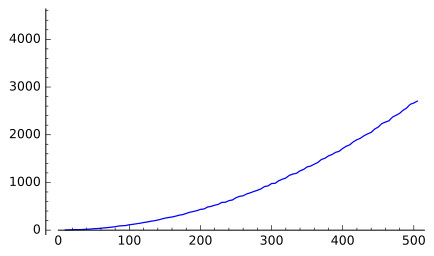
\includegraphics[width=0.8\textwidth]{./real.jpeg}
  \fbox{Gráfico del tiempo de ejecución de $100$ grafos connected\_watts\_strogatz\_graph}

  \caption{El grafo más pequeño es de 10 nodos y 20 aristas. El grafo más grande es de 505 nodos y 1010 aristas. }\label{fig:realWorld}
\end{figure}

\begin{figure}
  \centering
%   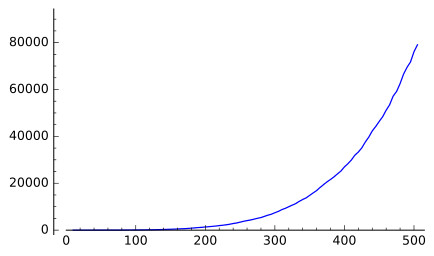
\includegraphics[width=0.8\textwidth]{./erdos2.jpeg}
  \fbox{Gráfico del tiempo de ejecución de $100$ grafos erdos\_renyi\_graph}

  \caption{El grafo más pequeño es de 10 nodos y 2 aristas. El grafo más grande es de 505 nodos y 4443 aristas. El tiempo máximo de ejecución es de 79088.2 ms, es decir, poco más de 13 minutos }\label{fig:erdos}
\end{figure}


\begin{figure}
  \centering
%   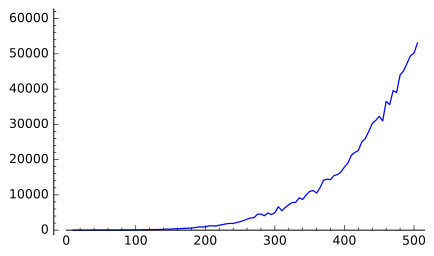
\includegraphics[width=0.8\textwidth]{./gnp2.jpeg}
  \fbox{Gráfico del tiempo de ejecución de $100$ grafos gnp\_random\_graph}

  \caption{El grafo más pequeño es de 10 nodos y 1 aristas. El grafo más grande es de 505 nodos y 1258 aristas. }\label{fig:gnp}
\end{figure}


\begin{figure}
  \centering
%   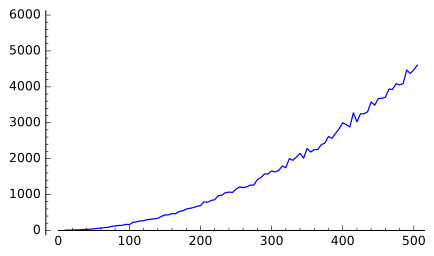
\includegraphics[width=0.8\textwidth]{./newman.jpeg}
  \fbox{Gráfico del tiempo de ejecución de $100$ newman\_watts\_strogatz\_graph}

  \caption{El grafo más pequeño es de 10 nodos y 29 aristas. El grafo más grande es de 505 nodos y 1322 aristas.El tiempo máximo de ejecución es de 4603.91 ms, es decir, alrededor de 7 minutos }\label{fig:newman}
\end{figure}



\end{document}
